根据前期的《软件需求规格说明书》和《软件工程总体设计报告》确定的功能模块,以及测试本身所设计到的方面,我们将从以下角度对该软件进行详细的测试。以下是测试内容的概览表格 表~\ref{xx}:

\begin{table}[h]
	\centering
	\begin{tabular}{|l|l|l|}
		\hline
		\textbf{测试项目名称} & \textbf{测试目的} & \textbf{测试内容} \\
		\hline
		面向对象测试 & 针对每一个类,测试是否设计正确 &  \\
		\hline
		功能验证测试 & 利用黑盒测试系统功能是否齐全,各个功能是否正确执行 & \textit{登录注册模块} \\
		& & \textit{个人中心模块} \\
		& & \textit{问诊预约模块} \\
		& & \textit{诊单账单模块} \\
		& & \textit{服务评价模块} \\
		\hline
		边界测试 & 测试程序对边界情况是否正确处理 & \textit{登录注册模块} \\
		& & \textit{个人中心模块} \\
		& & \textit{问诊预约模块} \\
		& & \textit{诊单账单模块} \\
		& & \textit{服务评价模块} \\
		\hline
		压力测试 & 测试系统在高负载情况下的功能和性能的承受情况 & \textit{登录注册} \\
		& & \textit{并发门诊预约} \\
		& & \textit{在线浏览门诊信息} \\
		& & \textit{查询历史记录} \\
		& &\textit{ 并发服务评价} \\
		\hline
		用户接口测试 & 测试用户能否通过网页界面完成想要执行的操作 &\textit{登录界面} \\
		& & \textit{注册界面} \\
		& & \textit{个人中心界面} \\
		& & \textit{问诊预约界面} \\
		& & \textit{诊单账单界面} \\
		& & \textit{服务评价界面} \\
		\hline
	\end{tabular}
	\caption{软件测试内容概览}\label{xx}
\end{table}

在接下来的测试文档中,我们将按照功能模块进行详尽的测试,确保每个模块都能满足预定的需求,并且能够在各种测试条件下稳定运行。测试将覆盖从面向对象设计的验证到功能验证、边界条件、压力测试以及用户接口的易用性等多个方面。通过这些全面的测试,我们能够确保软件的质量和可靠性,满足用户的需求,并提供流畅的用户体验。

\section{面向对象测试}
\subsection{系统整体架构}
\begin{figure}[htbp]
	\centering
	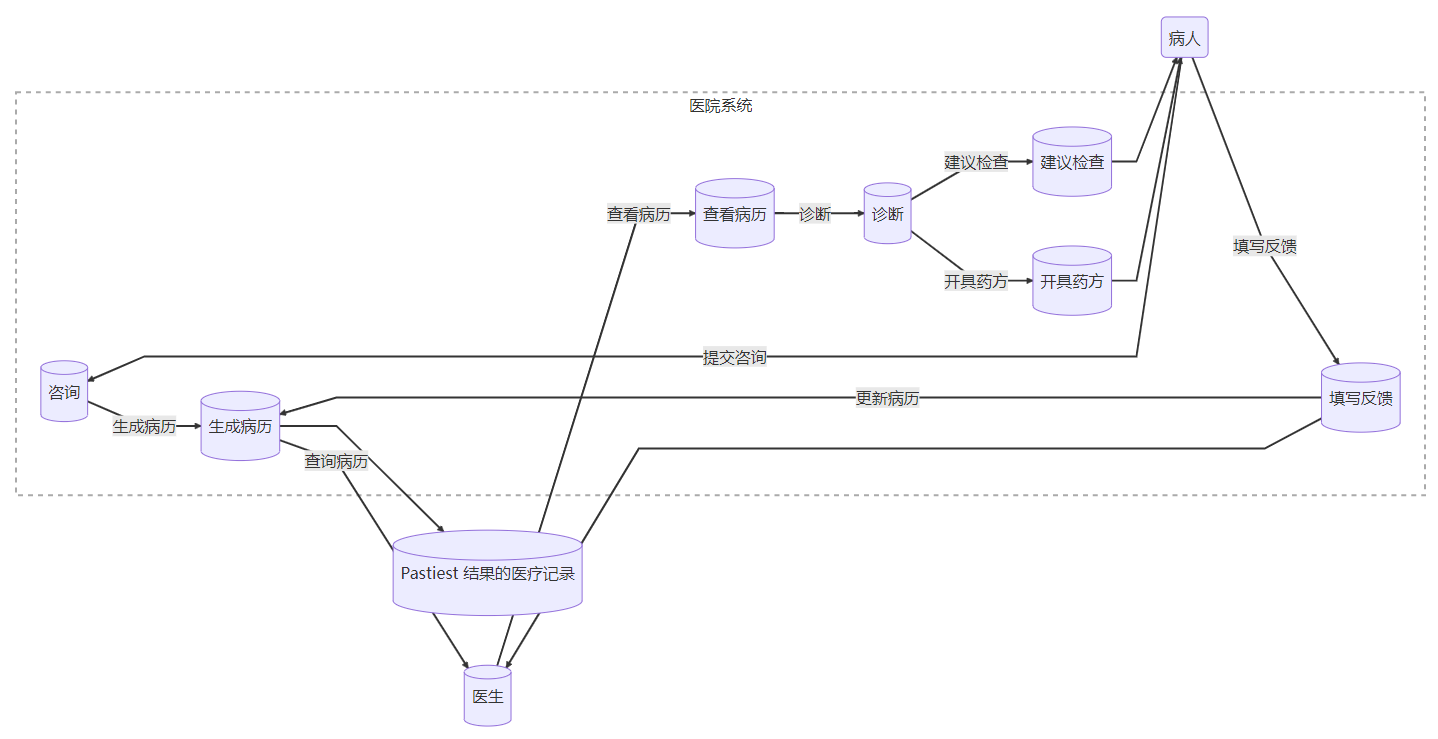
\includegraphics[width=\textwidth]{figures/sys.png}
	\caption{系统整体架构}
\end{figure}
我们小组主要实现的是前端部分
\begin{figure}[htbp]
	\centering
	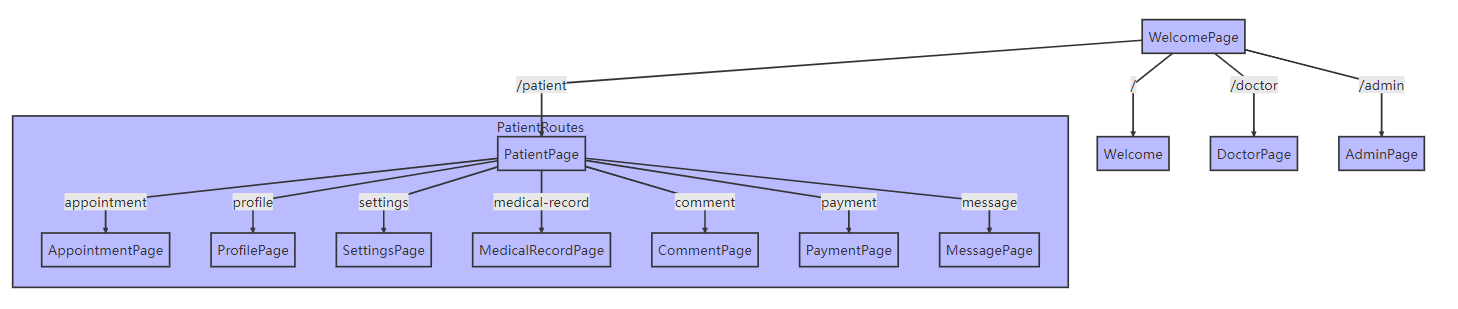
\includegraphics[width=\textwidth]{figures/front.png}
	\caption{前端整体架构}
\end{figure}
在我们的前端框架中,首页默认展示 WelcomePage,迎接用户的到来。患者相关的页面在 '/patient' 路径下,通过嵌套路由组织各个子页面,如预约、个人资料、设置、病历、评论、支付和消息,这些页面通过分层的方式提供了良好的用户体验和逻辑分组。此外,医生和管理员的页面分别通过 '/doctor' 和 '/admin' 路径访问,这些页面需要用户认证,确保只有授权用户才能访问,从而保障系统的安全性和数据的隐私性。通过这种设计,系统能够直观地满足不同角色用户的需求,提供高效和安全的操作体验。